\documentclass[a4paper,14pt]{article} % добrавить leqno в [] для нумерации слева
\usepackage{extsizes} % Возможность сделать 14-й шрифт

%%% Работа с русским языком
\usepackage{cmap}					% поиск в PDF
%\usepackage{mathtext} 				% русские буквы в фомулах
\usepackage[T2A]{fontenc}			% кодировка
\usepackage[utf8]{inputenc}			% кодировка исходного текста
\usepackage[english,russian]{babel}	% локализация и переносы
\usepackage{lipsum}                 % use \lipsum[1-4] \lipsum[] \lipum[2]
%///////////////////////////////////////////////////////////

% для красивых таблиц
\usepackage{booktabs}

%///////////////////////////////////////////////////////////

% для кастомизации списков
\usepackage{enumitem}
% \begin{itemize}[noitemsep,nolistsep]

%///////////////////////////////////////////////////////////

%%% Дополнительная работа с математикой
\usepackage{amsmath,amsfonts,amssymb,amsthm,mathtools} % AMS
\usepackage{icomma} % "Умная" запятая: $0,2$ --- число, $0, 2$ --- перечисление

\DeclarePairedDelimiter\abs{\lvert}{\rvert}%
\DeclarePairedDelimiter\norm{\lVert}{\rVert}%

\makeatletter
\let\oldabs\abs
\def\abs{\@ifstar{\oldabs}{\oldabs*}}
%
\let\oldnorm\norm
\def\norm{\@ifstar{\oldnorm}{\oldnorm*}}
\makeatother

%///////////////////////////////////////////////////////////

% активные ссылки
\usepackage[unicode]{hyperref}

% для кастомных ссылок 
\newcommand\myref[1]{\hyperref[#1]{#1}}

\usepackage{cleveref}

\hypersetup{
    colorlinks=true,
    linkcolor=blue,
    filecolor=magenta,      
    urlcolor=cyan,
    pdftitle={calculus},
    pdfpagemode=FullScreen,
    }

\urlstyle{same}

%///////////////////////////////////////////////////////////

%% Номера формул
\mathtoolsset{showonlyrefs=false} % Показывать номера только у тех формул, на которые есть \eqref{} в тексте.
%\usepackage{leqno} % Нумерация выражений слева

%///////////////////////////////////////////////////////////

%% Шрифты
\usepackage{euscript}	 % Шрифт Евклид
\usepackage{mathrsfs}    % Красивый матшрифт

%///////////////////////////////////////////////////////////

\usepackage{setspace} % Интерлиньяж
%\onehalfspacing % Интерлиньяж 1.5
%\doublespacing % Интерлиньяж 2
%\singlespacing % Интерлиньяж 1

%///////////////////////////////////////////////////////////

%% Перенос знаков в формулах (по Львовскому)
\newcommand*{\hm}[1]{#1\nobreak\discretionary{}
	{\hbox{$\mathsurround=0pt #1$}}{}}
	
%///////////////////////////////////////////////////////////

% bigcdot ( \cdot < \bigcdot < \bullet )
\usepackage{graphicx}
\graphicspath{ {./prints/} }

\makeatletter
\newcommand*\bigcdot{\mathpalette\bigcdot@{.5}}
\newcommand*\bigcdot@[2]{\mathbin{\vcenter{\hbox{\scalebox{#2}{$\m@th#1\bullet$}}}}}
\makeatother

%///////////////////////////////////////////////////////////

% Для обозначения множеств
\newcommand\sR{{\mathbb R}}
\newcommand\sQ{{\mathbb Q}}
\newcommand\sZ{{\mathbb Z}}
\newcommand\sN{{\mathbb N}}
% Для обозначения разбиения отрезка
\newcommand\sT{{\mathbb N}}
% Для обозначения отрезка $[a,b]$
\newcommand\ab{{$[a,b]$}}

%///////////////////////////////////////////////////////////


\usepackage{listings}
\usepackage{xcolor}
%New colors defined below
\definecolor{codegreen}{rgb}{0,0.6,0}
\definecolor{codegray}{rgb}{0.5,0.5,0.5}
\definecolor{codepurple}{rgb}{0.58,0,0.82}
\definecolor{backcolour}{rgb}{0.95,0.95,0.92}

%Code listing style named "mystyle"
\lstdefinestyle{mystyle}{
	backgroundcolor=\color{backcolour}, commentstyle=\color{codegreen},
	keywordstyle=\color{magenta},
	numberstyle=\tiny\color{codegray},
	stringstyle=\color{codepurple},
	basicstyle=\ttfamily\footnotesize,
	breakatwhitespace=false,         
	breaklines=true,                 
	captionpos=b,                    
	keepspaces=true,                 
	numbers=left,                    
	numbersep=5pt,                  
	showspaces=false,                
	showstringspaces=false,
	showtabs=false,                  
	tabsize=2
}

%"mystyle" code listing set
\lstset{style=mystyle}
\lstset{
	literate={а}{{\selectfont\char224}}1
	{б}{{\selectfont\char225}}1
	{в}{{\selectfont\char226}}1
	{г}{{\selectfont\char227}}1
	{д}{{\selectfont\char228}}1
	{е}{{\selectfont\char229}}1
	{ё}{{\"e}}1
	{ж}{{\selectfont\char230}}1
	{з}{{\selectfont\char231}}1
	{и}{{\selectfont\char232}}1
	{й}{{\selectfont\char233}}1
	{к}{{\selectfont\char234}}1
	{л}{{\selectfont\char235}}1
	{м}{{\selectfont\char236}}1
	{н}{{\selectfont\char237}}1
	{о}{{\selectfont\char238}}1
	{п}{{\selectfont\char239}}1
	{р}{{\selectfont\char240}}1
	{с}{{\selectfont\char241}}1
	{т}{{\selectfont\char242}}1
	{у}{{\selectfont\char243}}1
	{ф}{{\selectfont\char244}}1
	{х}{{\selectfont\char245}}1
	{ц}{{\selectfont\char246}}1
	{ч}{{\selectfont\char247}}1
	{ш}{{\selectfont\char248}}1
	{щ}{{\selectfont\char249}}1
	{ъ}{{\selectfont\char250}}1
	{ы}{{\selectfont\char251}}1
	{ь}{{\selectfont\char252}}1
	{э}{{\selectfont\char253}}1
	{ю}{{\selectfont\char254}}1
	{я}{{\selectfont\char255}}1
	{А}{{\selectfont\char192}}1
	{Б}{{\selectfont\char193}}1
	{В}{{\selectfont\char194}}1
	{Г}{{\selectfont\char195}}1
	{Д}{{\selectfont\char196}}1
	{Е}{{\selectfont\char197}}1
	{Ё}{{\"E}}1
	{Ж}{{\selectfont\char198}}1
	{З}{{\selectfont\char199}}1
	{И}{{\selectfont\char200}}1
	{Й}{{\selectfont\char201}}1
	{К}{{\selectfont\char202}}1
	{Л}{{\selectfont\char203}}1
	{М}{{\selectfont\char204}}1
	{Н}{{\selectfont\char205}}1
	{О}{{\selectfont\char206}}1
	{П}{{\selectfont\char207}}1
	{Р}{{\selectfont\char208}}1
	{С}{{\selectfont\char209}}1
	{Т}{{\selectfont\char210}}1
	{У}{{\selectfont\char211}}1
	{Ф}{{\selectfont\char212}}1
	{Х}{{\selectfont\char213}}1
	{Ц}{{\selectfont\char214}}1
	{Ч}{{\selectfont\char215}}1
	{Ш}{{\selectfont\char216}}1
	{Щ}{{\selectfont\char217}}1
	{Ъ}{{\selectfont\char218}}1
	{Ы}{{\selectfont\char219}}1
	{Ь}{{\selectfont\char220}}1
	{Э}{{\selectfont\char221}}1
	{Ю}{{\selectfont\char222}}1
	{Я}{{\selectfont\char223}}1
}

%///////////////////////////////////////////////////////////


%///////////////////////////////////////////////////////////

% Библиография
\usepackage{cite}
\usepackage{csquotes}
%\renewcommand{\refname}{Список источников}  % По умолчанию "Список литературы" (article)
%\renewcommand{\bibname}{Литература}  % По умолчанию "Литература" (book и report)

%///////////////////////////////////////////////////////////
%///////////////////////////////////////////////////////////
%///////////////////////////////////////////////////////////


%///////////////////////////////////////////////////////////

% squared itemize 
\newcounter{boxlblcounter}  
\newcommand{\makeboxlabel}[1]{\fbox{#1.}\hfill}% \hfill fills the label box
\newenvironment{boxlabel}
  {\begin{list}
    {\arabic{boxlblcounter}}
    {\usecounter{boxlblcounter}
     \setlength{\labelwidth}{3em}
     \setlength{\labelsep}{0em}
     \setlength{\itemsep}{2pt}
     \setlength{\leftmargin}{1.5cm}
     \setlength{\rightmargin}{2cm}
     \setlength{\itemindent}{0em} 
     \let\makelabel=\makeboxlabel
    }
  }
{\end{list}}

%///////////////////////////////////////////////////////////

%///////////////////////////////////////////////////////////

% Счетчик для теорем
\newcounter{counter_theorem}[section]
\setcounter{counter_theorem}{0}

% Счетчик для лемм
\newcounter{counter_lemma}[section]

% Счетчик для доказательств
\newcounter{counter_proof}[section]

% Счетчик для определений
\newcounter{counter_definition}[section]

% Счетчик для утверждений
\newcounter{counter_statement}[section]

%///////////////////////////////////////////////////////////

% Так можно задавать свою длину
\newlength{\mylength}
\settowidth{\mylength}{some text}
% \begin{minipage}{\mylength}
% {\textit{lipsum[1]}
% }
% \end{minipage}

%///////////////////////////////////////////////////////////

\newenvironment{title_theorem}[1]%
{%
    \addtocounter{counter_theorem}{1}%
    \noindent \textbf{Теорема \thesection.\arabic{counter_theorem}.}
    (#1) \newline \noindent%
}%
{\vspace{1cm}}

\newenvironment{not_title_theorem}%
{%
    \addtocounter{counter_theorem}{1}%
    \noindent \textbf{Теорема \thesection.\arabic{counter_theorem}.}
    \newline \noindent%
}%
{\vspace{1cm}}

\newtheorem{theorem}{Теорема}
\newtheorem{lemma}{Лемма}
\newtheorem{definition}{Определение}
\newtheorem{example}{Пример}
\newtheorem{consequence}{Следствие}
\newtheorem{statement}{Утверждение}


%///////////////////////////////////////////////////////////
%///////////////////////////////////////////////////////////
%///////////////////////////////////////////////////////////

\title{Математический анализ. Семестр 2} 
\author{Rustem Sirazetdinov}

\begin{document}
% 	\maketitle
	
	\newpage
	\tableofcontents
	
% 	\newpage
% 	\section*{Вступление}
%     \lipsum[1-3]
    
    % \noindent \newline
    % Если вы заметили ошибку, пожалуйста, напишите мне об этом: \url{avesirazetdinov@gmail.com} License: \textbf{WTFPL} 
    
    % \noindent
    % Особая благодарность следующим людям:
    % \begin{enumerate}
    %     \item Спасибо
    % \end{enumerate}
    
    %///////////////////////////////////////////////////////////
    %///////////////////////////////////////////////////////////
    
    \newpage
    \section{Неопределенный интеграл}
    \subsection{Первообразная}
    Наверное, свой рассказ я хочу начать с короткого вступления. Это вступление будет о первообразных. Далеее будут перечислены некоторые тривиальные для вас утверждения, просто для напоминания.
    
    
    \begin{definition}
    Функция $F(x)$ называется \textbf{первообразной} к функции $f(x)$ на некотором промежутке, если на этом промежутке функция $F$ дифференцируема и удовлетворяет уравнению $$F^\prime{}(x) = f(x)$$ или, что то же самое, соотношению $dF(x) = f(x)dx.$
    \end{definition}
    
    \noindent \( \bullet \) Операция перехода к перевообразной называется \textit{<<неопределенное интегрирование>>}, обозначается символом $\int f(x)dx$.
    
    \begin{statement}\label{st:dif_of_Antiderivatives}
    Если \(F_1(x)\) и \(F_2(x)\) - две первообразные к функции $f(x)$ на некотором промежутке I, то их разность $F_1(x) - F_2(x)$ на этом же промежутке I есть постоянная величина.
    \end{statement}
    
    $\blacksquare$  доказательство скоро появится, наверное... $\blacksquare$
    
    \bigskip
    \noindent Тогда из утрверждения \ref{st:dif_of_Antiderivatives} следует, что если $F(x)$ - какая-то производная к функции $f(x)$ на некотором промежутке $I$, то на этом промежутку $I$ верно: 
    \begin{equation}\label{eq:int_of_f(x)}
      \int f(x)dx = F(x) + C  
    \end{equation}
    другими словами любая первообразная может быть получена из конкретной $F(x)$ путем прибавления к ней некоторой постоянной.
    
    \begin{statement}
    Если \(F(x)\) некоторая первообразная к функции \(f(x)\) на некотором промежутке \(I\), то из \eqref{eq:int_of_f(x)} следует:
    \begin{equation}\label{eq:different_antider}
        \begin{boxed}
        {d\int f(x)dx = dF(x) = F^\prime{}(x)dx = f(x)dx}
        \end{boxed}
    \end{equation}
    но кроме того, поскольку неопределенный интеграл это любая из первообразных, то из \eqref{eq:int_of_f(x)} также следует, что
    \begin{equation}\label{eq:antider_of_differnt}
        \begin{boxed}
        {\int dF(x) = \int F^{\prime}(x)dx = F(x) + C.}
        \end{boxed}
    \end{equation}
    \end{statement}
    
    \noindent \textbf{Заключение}: формулы \eqref{eq:different_antider} и \eqref{eq:antider_of_differnt} показывают, что операции дифференцирование и неопределенного интегрирования взаимообратны с точностью до постоянной. 
    
    \subsubsection{Некоторые свойства первообразной}

    \begin{itemize}
        \item[\boxed{a.}]
            \begin{equation}\label{eq:lin_of_antiD}
                \int{(\alpha u(x) + \beta v(x))dx} = \alpha \int{u(x)dx} + \beta \int{v(x)dx}
            \end{equation}
        \item[\boxed{b.}]
            \begin{equation}\label{eq:multi_of_antiD}
                \int{(uv)'(x)dx} = \int{u'(x)v(x)dx} + \int{u(x)v'(x)dx}
            \end{equation}
        \item[\boxed{c.}] 
            \begin{itemize}
                \item[1.] \textbf{если} на некоторм промежутке \(I_x\) существует первообразная функции \(f(x)\), т.е. \(\int{f(x)dx} = F(x) + C\)
                
                \item[2.] \textbf{+} отображение \(\varphi : I_t \rightarrow I_x\) - гладкое\footnotemark{} отображение промежутка \(I_t\) в \(I_x\), то выполнено
            \end{itemize}
            \begin{equation}\label{eq:compose_of_antiD}
                \int{(f\circ\varphi)(t)\cdot\varphi'(t)dt} = (F\circ\varphi)(t) + C 
            \end{equation}
            
            
            \footnotetext{Отображение назвывает \textbf{гладким}, если оно непрерывно дифференцируемое. Зачем здесь нужна гладкость?}
    \end{itemize}
    
    \noindent $\blacksquare$ Равентсва \eqref{eq:lin_of_antiD}, \eqref{eq:multi_of_antiD}, \eqref{eq:compose_of_antiD} проверяются прямым дифференцированием их левой и правой частей. В \eqref{eq:lin_of_antiD} - свойство линейности дифференцирования; в \eqref{eq:multi_of_antiD} - дифференцирование произведения; в \eqref{eq:compose_of_antiD} - дифференцирование сложной функции. $\blacksquare$
    
    \bigskip
    \noindent Теперь перейдем к более практичным результатам, которые являются следствиями из полученных соотношений.
    
    \bigskip \noindent
    \eqref{eq:lin_of_antiD} \( \Rightarrow \) \textbf{линейность неопределенного интеграла}. Первообразную от линейной комбинации функций можно искать как линейнйую комбинацию первообразных этих функций.
    \[
    \int{\sum_{k=0}^{n} {a_{k}x^{k}}dx} = \sum_{k=0}^{n}{a_k \int{x^kdx}}
    \]
    
    \noindent
    \eqref{eq:multi_of_antiD} \( \Rightarrow \) \textbf{интегрирование по частям}. Формулу \eqref{eq:multi_of_antiD} в силу соотношения \eqref{eq:antider_of_differnt} можно переписать в виде 
    \[
    \int{u(x)dv(x)} = u(x)v(x) - \int{v(x)du(x)} + C
    \]
    Т.е. задачу нахождения первообразной функции \( u(x)v^\prime{}(x) \) можно свести к нахождению первообразной функции \( u^\prime{}(x)v(x). \)
    
    \bigskip \noindent
    \eqref{eq:compose_of_antiD} \( \Rightarrow \) \textbf{замена переменной в неопределенном интеграле}. При отыскании первообразной функции \( (f\circ\varphi)(t)\cdot\varphi^\prime{}(t) \) можно сначала произвести замену \( \varphi(t) = x \) под знаком интеграла и перейти к новой переменной \( x \), а после того как мы найдем первообразную как функцию от \( x \), вернемся обратно к старой переменной.
    
    \begin{eqnarray}
    \int{(f\circ\varphi)(t)\cdot\varphi^\prime{}(t) dt} = \int{f(\varphi(t))d\varphi(t)} = \int{f(x)dx} = F(x) + C = \nonumber \\ =  F(\varphi(t)) + C \nonumber
    \end{eqnarray}
    
    
    
    \subsection{Основные общие приемы отыскания первообразной}
    
    \begin{center}
        \href{https://miro.com/app/board/uXjVOHbcyR4=/?invite_link_id=437398013079}{ссылка на доску}
    \end{center}
    
    \subsection[Метод Остроградского]{Метод Остроградского выделения рациональной части интеграла от правильной рациональной дроби}
    
    \noindent Пусть \( \frac{P(x)}{Q(x)}\) - правильная рациональная дробь; \( q(x) \) - многочлен, имеющий те же корни, что и \( Q(x) \), но каждый из них имеет кратность 1 и тогда \( Q_1(x) = \frac{Q(x)}{q(x)}. \) В таком случае имеет место формула Остроградского: 
    \[
    \int{\frac{P(x)}{Q(x)}dx} = \frac{P_1(x)}{Q_1(x)} + \int{\frac{p(x)}{q(x)}dx,}
    \]
    где \(\frac{P_1(x)}{Q_1(x)}\ \text{и}\ \frac{p(x)}{q(x)} \) - рациональные дроби, причем \( \int{\frac{p(x)}{q(x)}dx} \) - трансцендентная функция. 
    
    
    \section{Определенный итеграл}
    \setcounter{equation}{0}
    
	Основная задача интегралов - нахождение первообразной. Зная первообразную функции, с помощью формулы Ньютона-Лейбница можно найти площадь под графиком этой функции.
	
	\subsection{Формула Ньютона-Лейбница}
	
	Здесь я приведу рассуждение, наводящее на формулу Ньютона\\-Лейбница, его идея лежит в основе интеграла Римана.
	
	\vspace{0.5cm}
	Пусть точка движется вдоль числовой оси, \( s(t) \) - её координата в момент \( t \), а \( v(t) = s^\prime{}(t) \) - её скорость в тот же момент \( t \). Предположим, что мы значем положение \( s(t_0) \) точки в момент \( t_0 \) и то, как со временем изменяется скорость. Зная все это, мы хотим научится вычислять \( s(t) \) для любого фиксированного значения \( t > t_0 \).
	
	Если считать, что скорость \( v(t) \) меняется непрерывно, то смещение точки за малый промежуток времени можно приближенно вычислять как произведение \( v(\tau)\Delta t \) скорости в произвольный момент времени промежутка \( \tau \) на длину этого промежутка. Тогда разобьем весь отрезок \( [t_0, t] \),  отметив некоторые моменты времени \( t_i (i = 0,\dots,n) \), так, что \( t_0 < t_1 < \dots < t_n = t \) ,и так, что промежутки \( [t_{k-1}, t_{k}] \) достаточно малы. Теперь пусть \( \Delta t_i = t_i - t_{i-1} \) и \( \tau_i \in [t_{i-1}, t] \), тогда имеем приближенное равенство 
	\[
	s(t) - s(t_0) \approx \sum_{i=1}^{n} {v(\tau_i)\Delta t_i}.
	\]
	Это приближенное равеноство будет тем точнее, чем меньше промежутки разбиения, а значит в пределе, когда величина \( \lambda \) наибольшего из промежутков разбиения стремится к нулю, получим точное равенство
	\begin{equation}\label{eq:FTC_physics}
	    \lim_{\lambda\to 0}{\sum_{i=1}^{n}{v(\tau_i)\Delta t_i} = s(t) - s(t_0)}.
	\end{equation}
	
	Это равенство и называется \textbf{формулой Ньютона-Лейбница} или \href{https://en.wikipedia.org/wiki/Fundamental_theorem_of_calculus}{фундаментальной теоремой математического анализа}. 
	
	\subsection{Введение в интеграл Римана}
	Давайте попробуем посчитать площадь. Например посчитаем площадь под параболой \( y=x^2 \) над отрезком \( [0, 1] \). Будем считать эту площадь методом исчерпания фигуры посредством простейших фигур - прямоугольников.
	Разобьём отрезок \( [0, 1] \) точками \( 0=x_0 < x_1 < \dots < x_n = 1 \) на достаточно мелкие отрезки \( [x_{i-1}, x_i] \).
	
	\begin{figure}[h]
	\centering
    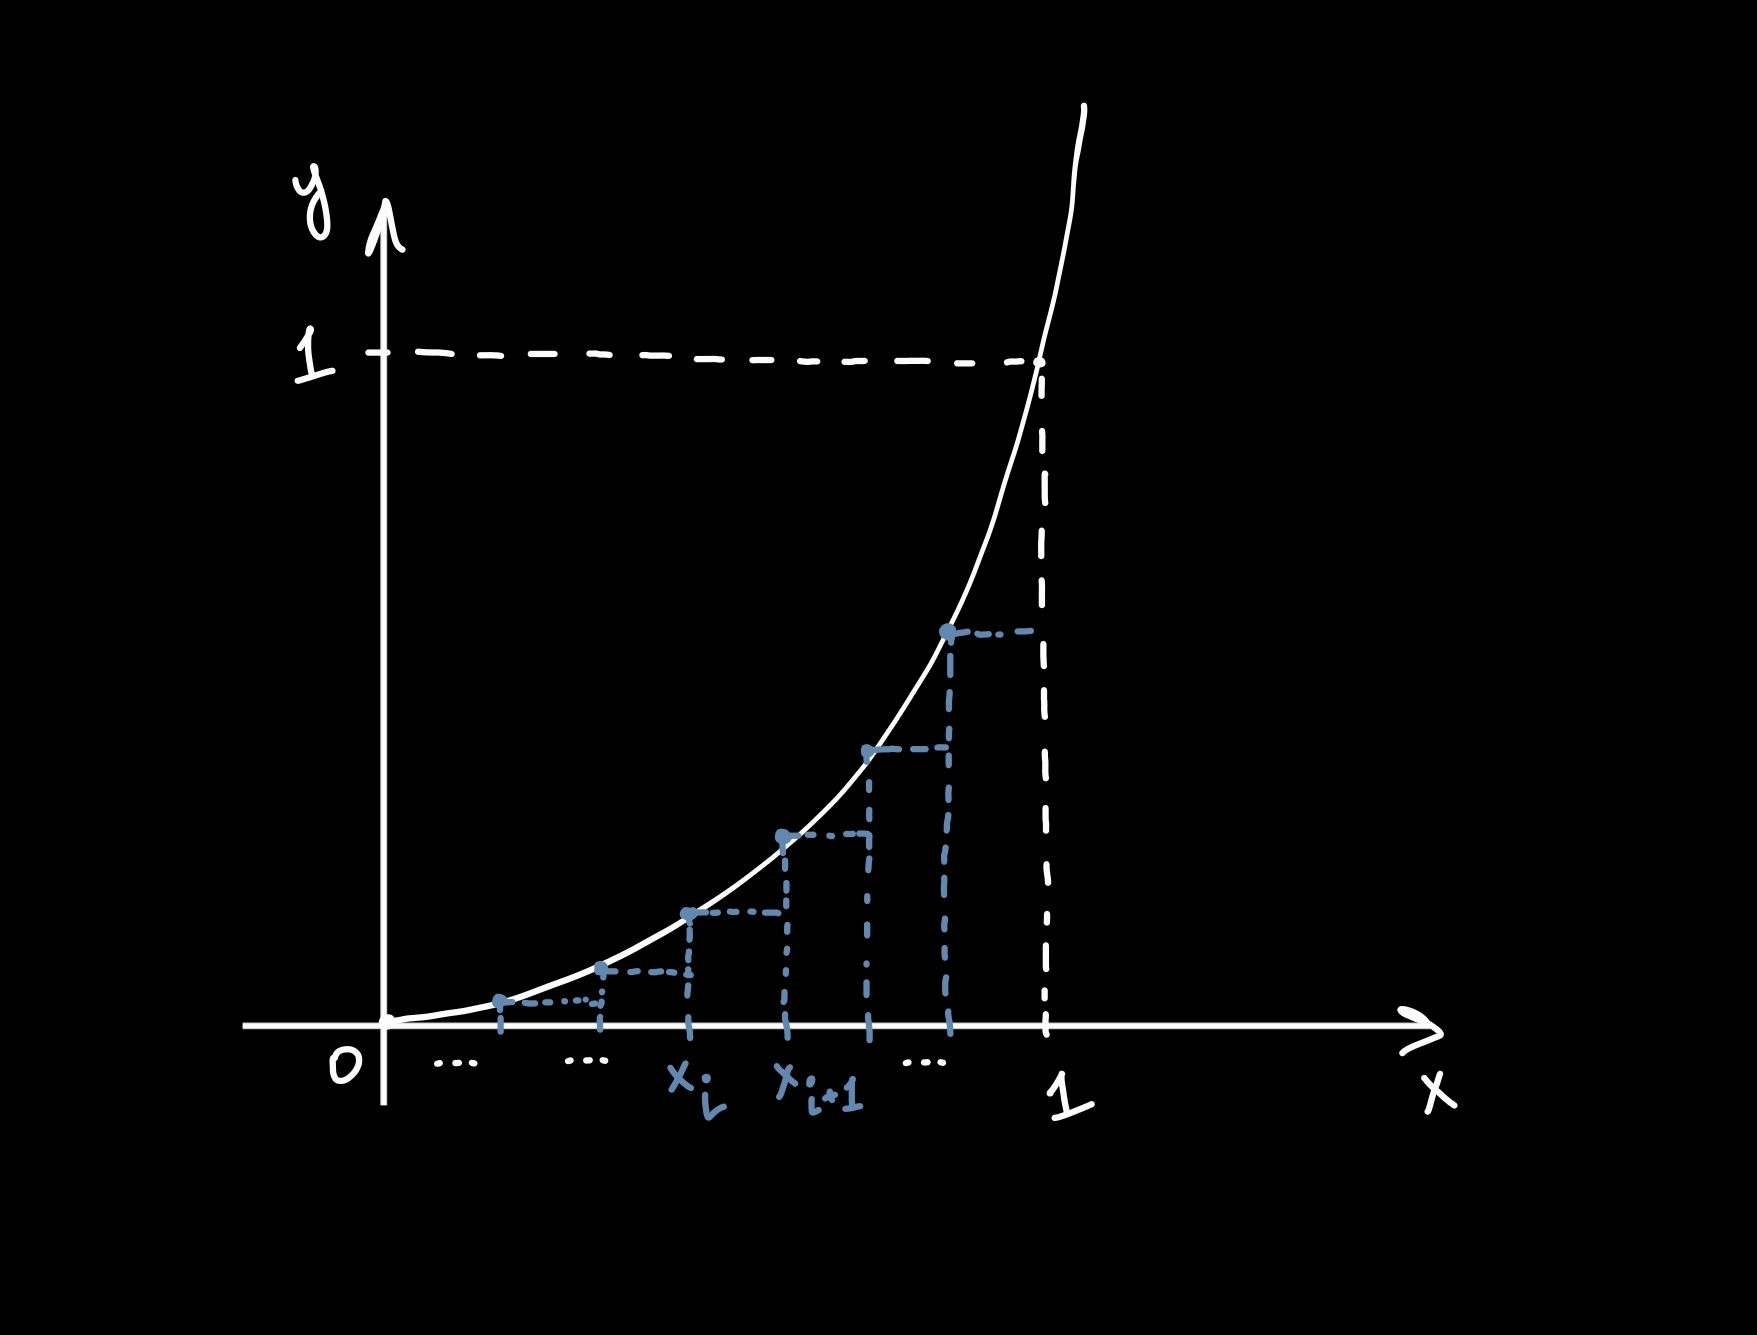
\includegraphics[width=5cm, height=4.5cm]{Integral_of_Archimedes.jpg}
    \caption{Убогий рисунок}
    \end{figure}
	
	\noindent 
	Теперь мы сможем приблизительно вычислить площадь \( \sigma \) как сумму площадей изображенных на рисунке прямоугольников:
	\[
	\sigma \approx \sum_{i=1}^{n}{x_{i-1}^{2}\Delta x_i}
	\]
	Отойдем в сторону, пусть \(f(x) = x^2 \) и \( \xi_i=x_{i-1} \), тогда полученная формула перепишется в виде 
	\begin{equation}\label{eq:for_integral_sum}
	    \sigma \approx \sum_{i=1}^{n}{f(\xi_i)\Delta x_i}.
	\end{equation}

	И переходя к пределу в итоге будем иметь
	\begin{equation}\label{eq:yeet}
	    \lim_{\lambda\to 0}{\sum_{i=1}^{n}{f(\xi_i)\Delta x_i}} = \sigma.
	\end{equation}
	
	\noindent
	Формула \eqref{eq:yeet} только обозначениями отличается от формулы \eqref{eq:FTC_physics}. Забыв о геометрическом смысле \(f(\xi) \), \( \Delta x_i \) и считая \( x \) временем, а \(f(x) \) cкоростью, найдем первообразную \( F(x) \) функции \(f(x) \) и тогда по формуле \eqref{eq:FTC_physics} получим, что о с кепкой равно \( F(1) - F(0) \)
	
	
	\subsection{Определение интеграла Римана}
	\subsubsection[Разбиения]{Разбиения. База в множестве разбиений}
	
	\setlength{\parindent}{0pt}
	
    При подсчете площади под графиком параболы на отрезке $[0, 1]$ 
	мы разбили этот отрезок точками \( 0=x_0 < x_1 < \dots < x_n = 1 \) на подходящие нам отрезки, т.е. мы предъявили некоторое разбиение отрезка, которое <<подошло для конкретной задачи>>. Теперь опрделим понятие разбиения.
	
	\begin{definition}
	\textbf{Разбиением \( \mathbb{T} \) }(или обозначают \(P\)) отрезка \( [a, b], a < b,\) называется такая конечная (и абсолютно произвольная) система точек \( x_0, \dots , x_n \) этого отрезка (точки должны принадлежать отрезку в случае, если отрезок не линейно связное множество\footnotemark{}), что \( a = x_0 < x_1 < \dots < x_n = b \).
	
	\textbf{Диаметром} (или параметром, или нормой) разбиения назывется максимум \( \lambda(\mathbb{T}) \) из длин отрезков разбиения.
	\end{definition}
	
	\footnotetext{Пространство называется линейно связным, если любые две его точки можно соеденить \textbf{непрерывной} кривой}
	
	Такое обычное разбиение отрезка дальше не будет представлят интерес, более важное понятие - разбиение отрезка с отмеченными точками.
	
	\begin{definition}
	Говорят, что имеется \textbf{разбиение} \(( \mathbb{T}, \xi )\) \textbf{с отмеченными точками} отрезка \( [a, b], a < b,\) если имеется разбиение $ \mathbb{T} $ этого отрезка и в каждом из отрезков разбиения \( [x_{i-1}, x_i] \) абсолютно произвольно выбрана точка $ \xi_i \in [x_{i-1}, x_i]. $ 
	\end{definition}
	
	\begin{figure}[h]
	\centering
    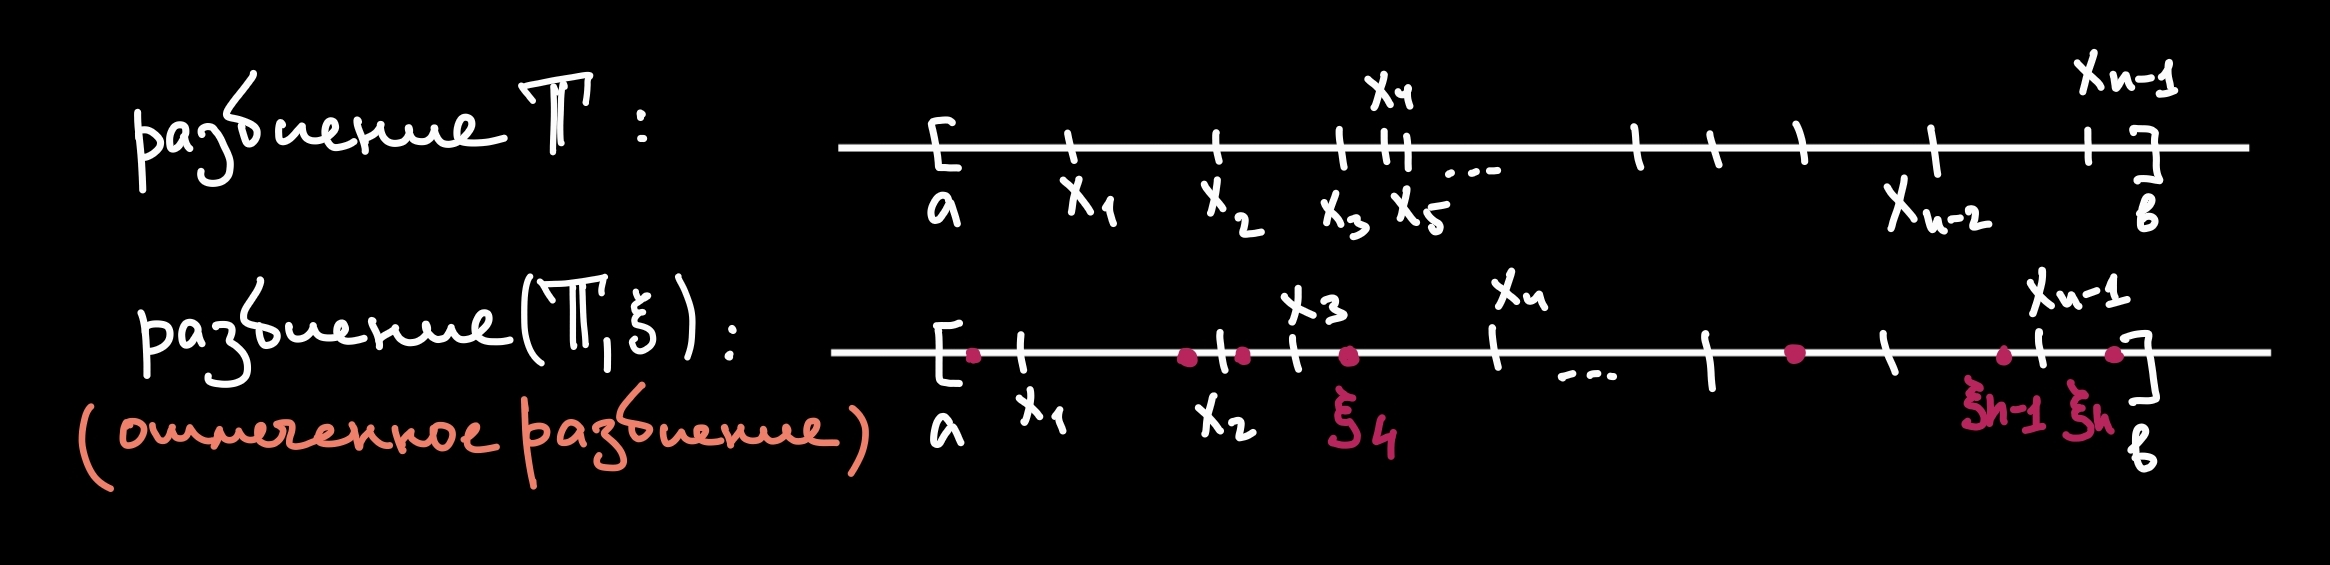
\includegraphics[width=\textwidth, height=4.5cm]{Partition_of_an_interval.jpg}
    \caption{Разбиение и разбиение с отмеченными точками отрезка}
    \end{figure}
	
	Чуть позже мы постоянно будем пользоваться этим понятием.
	
	\bigskip
	Теперь рассмотрим базу $ \mathscr{B} = {B_d} $ в множестве $ \mathscr{P} $ разбиений с отмеченными точками данного отрезка \( [a, b], a < b,\). Пусть элемент $ B_d, d > 0 $ базы $ \mathscr{B} $ есть совокупность всех тех разбиений \(( \mathbb{T}, \xi )\) с отмеченными точками отрезка \( [a, b] \), для которых $ \lambda(\mathbb{T}) < d $.
	
	\smallskip
	Проверим, что $ {B_d}, d> 0$ -- действительно база в множестве $ \mathcal{P} $.
	
	$\blacksquare \RHD \LHD \medbullet ... \blacksquare $
	
	\subsubsection{Интегральная сумма}
	
	Введем еще одно очень важное для определения интеграла Римана понятие.
	\begin{definition}
    Если
    \begin{enumerate}
        \item {функция \(f\) определена на отрезке \( [a, b] \) }
        \item {\(( \mathbb{T}, \xi )\) разбиение с отмеченными точками этого отрезка, то сумма }
    \end{enumerate}
    \begin{equation}\label{def:integral_sum}
        \sigma(f;\mathbb{T}; \xi) \\mathrel{\mathop:}=qq \sum_{i=1}^{n}{f(\xi_i)\Delta x_i,} 
    \end{equation}
    где $ \Delta x_i = x_i - x_{i-1} $, называется \textbf{интегральной суммой} функции $f$ соответсвующей разбиению \(( \mathbb{T}, \xi )\) отрезка \( [a, b] \).
	\end{definition}
	
	Теперь, когда мы определили важные понятия и доказали существования базы $ \mathscr{B} $ в $\mathscr{P} $ можно ставить вопрос о пределе некоторой функции $ \sigma(f;\mathbb{T}; \xi). $ Почему нам интересен предел мы выясним позже, но если неймется, то именно через интегральные суммы можно считать площадь под графиком <<некоторых>>\footnotemark{} функций, а вычисление площади под графиком это основная идея интегралов. 
	\footnotetext{далеко не всех}
	
	\subsubsection{Интеграл Римана}
	
	Для начала ответим на вопроc, почему сумма \eqref{def:integral_sum} называется интегральной. Снова обратимся к примеру подсчета площади под парбалой на отрезке \( [0,1] \). Суммы \eqref{eq:for_integral_sum} и \eqref{def:integral_sum} на самом деле очень похожи. В каждой из них выражение, стоящее под знаком суммы, есть произведение значения функции в конкретной точке определенного отрезка на длину этого же отрезка, в первом случае мы отождествили это с площадью прямоугольнка, расположенного под дугой параболы, высота которого равна значению функции $f$ в точке $\xi_i$, а ширина равна длине отрезка $ \Delta x_i = x_i - x_{i-1} \ni \xi_i$, суммой таких прямоугольников мы хотели приблизить значение площади под параболой, далее мы будем заниматься именно этим. Будем приближать значение площади под графиком некоторой функции столбиками, поэтому эти суммы и называются интегральными. Но наши суммы будут тем точнее, чем меньше диаметр разбиения, т.е. нам необходимо диаметр \( \lambda(\mathbb{T}) \) разбиения \( \mathbb{T} \) устремить к 0, т.е. перейти к пределу. Теперь связь между интегральными суммами и итегралом Римана должна стать очевидной. Кроме того, существуеют и другие идейно не похожие на интеграл Римана способы вычисления площади.
	
	\bigskip
	Теперь представим классическое определение интеграла Римана. Пусть $f$ -- функция, заданная на отрезке \( [a, b] \).
	\begin{definition}\label{def:1def_of_Rintegral}
	    Говорят, что число \textbf{$I$} является \textbf{интегралом Римана} от функции $f$ на отрезке \( [a, b] \), если для любого $ \varepsilon > 0 $ найдется такое число \( \delta > 0 \) такое, что для любого разбиения \(( \mathbb{T}, \xi )\), диаметр которого \( \lambda(\mathbb{T}) < \delta \), верно соотношение 
	    \[
	    \abs{ I - \sum_{i=1}^{n}{f(\xi_i)\Delta x_i}} < \varepsilon.
	    \]
	\end{definition}
	Это опрделение практически в точности повторяет опрделение предела функции, так и должно быть ведь \(\sigma(f;\mathbb{T}; \xi)\) при фиксированной функции $f$ можно считать как функцию \( \Phi(\mathbb{T}; \xi) \) от разбиения \(( \mathbb{T}, \xi )\). 
    % “def =” (\stackrel{\text{\tiny def}}{=}
    Поскольку ранее мы определили базу $\mathscr{B}$ в множестве разбиений $ \mathscr{P}$, а разбиения $ p = ( \mathbb{T}, \xi ) $, для которых \( \lambda(\mathbb{T}) < \delta \), составляют элемент этой базы $B_d$, то определение \ref{def:1def_of_Rintegral} равносильно тому, что 
    \[
    I = \lim_{\mathscr{B}}{\Phi(p)},
    \]
    \textbf{т.е. интеграл $I$ есть предел по базе $\mathscr{B}$ значений интегральных сумм функции $f$.} Теперь естественно обозначить базу $\mathscr{B}$ символом $\lambda(\mathbb{T}) \to 0 $, и тогда получим окончательное определение:
    \begin{equation}\label{def:main_def_of_Rintegral}
    \begin{boxed}
        {\int_{a}^{b}{f(x)dx} \\mathrel{\mathop:}=qq \lim_{\lambda(\mathbb{T}) \to 0}{\sum_{i=1}^{n}{f(\xi_i)\Delta x_i}}}
    \end{boxed}
    \end{equation}
    
   \begin{definition}
        Функция $f$ называется интегрируемой по Риману на отрезке $[a,b]$, если для нее существует указанный в \eqref{def:main_def_of_Rintegral} предел интегральных сумм при $\lambda(\mathbb{T}) \to 0$(т.е. если для нее определен интеграл Римана)
   \end{definition}
   Множестве функций интегрируемых по Риману будем обозначать через $\mathscr{R}[a,b].$
   
   \subsection{Условия интегрируемости по Риману}
    Поскольку интегрируемость функции $f$ на отрезке $[a,b]$ зависит от наличия предела некторой функции $\sigma(f;\mathbb{T};\xi)$, то пользуясь критерием Коши существования предела функции, определим необходимое и достаточное условие интегрируемости функции. Напомним суть критерия Коши.
    
    \bigskip
    \textsc{Первая формулировка.}
    Пусть $X$ - множество и $\mathscr{B}$ - база в множестве $X$ 
    Функция $f : X \to \mathbb{R} $ имеет предел по базе $\mathscr{B}$ тогда и только тогда, когда для любого (сколь угодно малого наперед заданного) числа \(\varepsilon > 0\) найдется элемент $B \in \mathscr{B}$ базы, на котором колебание функции меньше $\varepsilon$.
    
    \bigskip
    \textsc{Вторая формулировка.} Функция $f : X \to \mathbb{R} $ имеет предел при \( x \rightarrow a \) тогда и только тогда, когда когда для любого числа \(\varepsilon > 0\) найдется такое число \(\delta > 0\), что для любых точек \(x_1\) и \(x_2\) из проколотой окретсности \( \mathring{U}_{E}^{\delta}(a) \) выполнено \[ \abs{f(x_1) - f(x_2)} < \varepsilon. \] 
    
    \textit{Колебанием функции} \( f : X \to \mathbb{R} \) на множестве \(E\subset X\) называется величина \[ \omega (f;E) \\mathrel{\mathop:}=qq \sup_{x_1,x_2 \in E}{\abs{f(x_1) - f(x_2)}} \]
    
    Теперь можно сказать, что функция \(f\) интегрируема на отрезке \([a,b]\) тогда и только тогда, когда для любого \(\varepsilon > 0\) найдется \(\delta > 0\) такое, что для любых разбиений \(( \mathbb{T}', \xi' )\) и \(( \mathbb{T}'', \xi'' )\)  отрезка \([a,b]\) выполнено неравенство
    \[
    \abs{\sigma(f;\mathbb{T}'; \xi' - \sigma(f;\mathbb{T}''; \xi'')} < \varepsilon
    \]
    или, что тоже самое 
    \begin{equation}\label{eq::Cauchy's_criteria}
        \abs{\sum_{i=1}^{n'}{f(\xi_{i}')\Delta x_{i}'} - \sum_{i=1}^{n''}{f(\xi_{i}'')\Delta x_{i}''}} < \varepsilon.
    \end{equation}
    
    Сейчас мы получили некоторый результат, один из критериев интегририруемости функции по Римана на отрезке, но этот результат не очень удобен на практике, ведь его проверка достаточно трудоемное дело, но этот результат важен как для понимая, так и для постороения условий интегрируемости.
    
    \subsubsection{Первое необходимое условие интегрируемости}
    \begin{statement}
    Для того чтобы функция \(f\), определенная на отрезке \([a,b]\), была интегрируемой по Риману на нем, необходимо, чтобы она была ограничена на этом отрезке.
    \[
    (f \in \mathscr{R}[a,b]) \Rightarrow ( f\ \textnormal{ограничена на}\ [a,b]).
    \]
    \end{statement}
    
    \( \blacksquare \dots \blacksquare \)
    
    \subsubsection{Первое достаточное условие интегрируемости}
    \begin{statement}\label{st:1dos_Rintegral}
    Для того чтобы ограниченнаяна отрезке \([a,b]\) функция \(f\) была интегрируемой по Риману на нем, достаточно, чтобы для любого числа \(\varepsilon > 0\) найдется число \(\delta > 0\) такое, что при любом разбиении \(\mathbb{T}\) отрезка \( [a,b] \) с параметром \(\lambda(\mathscr{T}) < 0\) выполнялось соотношение
    \[
    \sum_{i=1}^{n}{\omega(f;\Delta_i)\Delta x_i} < \varepsilon.
    \]
    
    \end{statement}
    
    \(\blacksquare \dots \blacksquare \)
    
    Утверждение \ref{st:1dos_Rintegral} на первый взгяд очень похоже на критерий Коши \eqref{eq::Cauchy's_criteria}, что мы приводили ранее, конечно, это правда ведь достаточное условие одна из составляющих этого критерия. Давайте теперь разберемся как приведенные условия образуют вместе критерий Коши.(об этом будет подробно в будущем док-ве)
    
    
    Что нам говорит критерий Коши? Что интегральная сумма не зависит от разбиения отрезка. При разных разбиениях интегральные суммы отличаются лишь на некоторое число \(\varepsilon > 0\). Ок, что нам дает достаточное условие? При любых \(\varepsilon > 0\) и  разбиении колебания функции на каждом из отрезков не больше \(\varepsilon\) (т.е. значения функции на каждом из отрезков достаточно мало отличаются друг от друга), тогда   Начнем с необходимого условия. Если функция не будет ограничена хотя бы на одном отрезке, то для любого разбиения интегралтная сумма будет неограниченной, тогда у нас никак не может выполниться неравенство \eqref{eq::Cauchy's_criteria}.
    
    Теперь определим роль достаточного условия. Если функция удовлетворяет достаточному условию, то по любому числу \(\varepsilon > 0\) можно найти число \(\delta > 0\) так, что для любого разбиения \(\mathbb{T}\) отрезка \( [a,b] \) с параметром \(\lambda(\mathbb{T}) < \delta\) ...  не знаю как дальше написать, в доказательстве все разбру.
    
    
    \begin{consequence}
    Любая непрерывная на отрезке функция интегрируема по Риману на этом отрезке, т.е.
    \[
    (f \in C[a,b]) \Rightarrow (f \in \mathscr{R}[a,b]).
    \]
    \end{consequence}
    
    \(\blacksquare \dots \blacksquare\)
    
    \begin{consequence}
    \textnormal{
    Если ограниченная на отрезке \( [a,b] \) функция \(f\) непрерына на этом отрезке всюду, кроме быть может, конечного множества точек, то \(f \in \mathscr{R}[a,b].\)
    }
    \end{consequence}
    
    \(\blacksquare \dots \blacksquare\)
    
    \begin{consequence}\label{conseq:monotonic}
    Монотонная на отрезке функция интегрируема на этом отрезке. 
    \end{consequence} 
    
    \(\blacksquare \dots \blacksquare\) 
    
    \textsc{\textbf{Замечание 1.}} Монотонность определена \textbf{только} для вещественнозначных функций одной переменной. Почему? Функции нескольких переменных задают плоскости и поверхности в пространстве. Для определенности будем считать, что функция от двух переменных. В общем случае она задает какую-то плоскость(если вся плоскость - константа, то про монотонность теряет смысл, ведь суть монотонности, в том, что зная признаки монотонность, мы можем узнать как будут меняться значения функции, тогда будем считаь, что задана не совсем тривиальная плоскость - поверхность.) Пусть точка $M(x,y)$ - некоторая точка в плоскости $XOY$, тогда проведем через точку M две пересекающиеся прямые. Тогда вдоль одной прямой значения будут возрастать, а вдоль другой убывать, т.е. нельзя однозначно определить монотонность.
    
    \bigskip
    \textsc{\textbf{Замечание 2.}} До этого момента мы всегда работали с вещественнозначными функциями, но мы НИГДЕ(кроме следствия \ref{conseq:monotonic}) не пользовались свойствами вещественно значных функций, поэтому все выше сказанное можно обобщить на коплексно- или векторнозначные функции. А теперь мы перейдем к сюжету, который специфичен только для функций с вещественными значениями. 
    
    \begin{definition}
         Пусть \( f : [a,b] \rightarrow \texthbb{R} \) - вещественнозначная фукнция определнная и \textbf{ограниченнная} на отрезке \([a,b]\)\textnormal{;} $\mathbb{T}$ - разбиение отрезка \([a,b]\)\textnormal{;} \(\Delta_i \ (i = 1,\dots,n)\) - отрезки разбиения. Положим, что 
         \[ 
        m_i = \adjustlimits \inf_{x \in \Delta_i}{f(x)}, \ M_i = \adjustlimits \sup_{x \in \Delta_i}{f(x)} \ (i = 1,\dots,n)
         \]
        Суммы 
        \[
        s(f;\mathbb{T}) \mathrel{\mathop:}= \sum_{i=1}^{n}{m_i\Delta x_i}
        \]
        и
        \[
        S(f;\mathbb{T}) \mathrel{\mathop:}= \sum_{i=1}^{n}{M_i\Delta x_i}
        \]
        называются \textbf{нижней и верхней суммой Дарбу}.
    \end{definition}
    
    Если \( (\mathbb{T}, \xi) \) - произвольное разбиение отрезка \( [a,b] \), то выполненено неравентсво
    \begin{equation}\label{ineq:Интегральная сумма заключена между инфинумом и супремумом.}
        s(f;\mathbb{T}) \leqslant \sigma(f;\mathbb{T};\xi) \leqslant S(f;\mathbb{T})
    \end{equation}
    
    \begin{lemma}\label{eq:lemma1}
    \[
    s(f;\mathbb{T}) = \inf_{\xi}{\sigma(f;\mathbb{T};\xi)}, \ \  S(f;\mathbb{T}) = \sup_{\xi}{\sigma(f;\mathbb{T};\xi)}
    \]
    \end{lemma}
    \(\blacksquare \dots \blacksquare\) 
    
    Как итог леммы \ref{eq:lemma1} и неравенства \eqref{ineq:Интегральная сумма заключена между инфинумом и супремумом.} получим критерий интергируемсти вещественнозначной функции.
    
    \begin{theorem}
    \textbf{\textsc{(Критерий Дарбу)}} \textbf{Ограниченная вещественнозначная функция} $f : [a,b] \rightarrow \mathbb{R}$ интегрируема по Риману на отрезке $[a,b]$ тогда и только тогда, когда существуют и равны между сабой пределы 
    \begin{equation}
    \underline{\textnormal{I}} = \lim_{\lambda(\mathbb{T}) \rightarrow 0}{s(f;\mathbb{T})}, \ \ \overline{\textnormal{I}} = \lim_{\lambda(\mathbb{T}) \rightarrow 0}{S(f;\mathbb{T})}    
    \end{equation}
    При этом их общее значение $\textnormal{I} = \underline{\textnormal{I}} = \overline{\textnormal{I}}$ совпадает с интегралом 
    \[
    \int_{a}^{b}{f(x)dx}
    \]
    \end{theorem}
    
    \(\blacksquare \dots \blacksquare\) 
    
    \begin{statement}
    Для того чтобы функция $f : [a,b] \rightarrow \mathbb{R}$ была интегрируема по Риману \textbf{необходимо и достаточно} выполнение соотношения
    \begin{equation}
        \lim_{\lambda(\mathbb{T}) \rightarrow 0}{\sum_{i=1}^{n}{\omega(f;\Delta_i)\Delta x_i}} = 0
    \end{equation}
    \end{statement}
    
    \(\blacksquare \dots \blacksquare\) 
    
    \section[Критерий Лебега]{Критерий Лебега интегрируемости функции по Риману}
    Наконц-то переходим к ключевому сюжету, который дает внутреннее описание интегрируемой по Риману функции.
    
    
\end{document}